\documentclass[../cheatSheetAlgoritmi.tex]{subfiles}
\begin{document}

\section{Programmazione Greedy}
\subsection{Introduzione}
Nella sezione precedente ci siamo occupati di risolvere alcuni problemi mediante l'utilizzo di programmazione dinamica e, in alcuni di questi casi, abbiamo dovuto controllare tutte le possibili soluzioni ottenute poiché non eravamo certi di dove potesse trovarsi il risultato. In questo capitolo ci occuperemo invece della programmazione greedy e ciò di selezionare una sola tra le scelte possibili, quella che ci sembra la migliore (localmente ottima), dimostrando però che questa scelta si rivela poi essere ottima a livello globale.\\
\textbf{ATTENZIONE:} Non tutti i problemi hanno una scelta ingorda come soluzione!
\subsection{Insieme indipendente massimale di intervalli}
\textbf{Input}\\
Sia $S$ = $\{1, 2, ..., n\}$ un insieme di intervalli della retta reale. Ogni intervallo $[a_i, b_i]$ con $i \in S$, è chiuso a sinistra e aperto a destra.
\begin{itemize}
	\item  $a_i:$ \textcolor{red}{tempo di inizio}
	\item  $b_i:$ \textcolor{red}{tempo di fine}
\end{itemize}
\textbf{Definizione del Problema} \\
Un \textcolor{red}{insieme indipendente massimale} è un sottoinsieme di massima cardinalità formato da intervalli tutti disgiunti tra loro.
\subsubsection{Dalla programmazione dinamica...}
Prima di parlare della risoluzione del problema con la tecnica greedy proviamo a vedere come avremmo affrontato il problema con programmazione dinamica, definendo la sottostruttura ottima, per cercare la cosiddetta scelta ingorda.\\\\
\textbf{Sottostruttura Ottima}\\
Si assuma che gli intervalli siano ordinati per tempo di fine: $b_1 \leq b_2 \leq ... \leq b_n$\\
Definiamo il \textcolor{red}{sottoproblema $S[i...j]$} come l'insieme di intervalli che iniziano dopo la fine di $i$ e finiscono prima dell'inizio di $j$: $S[i...j] = \{k|b_i \leq a_k < b_k \leq a_j\}$\\
Aggiungiamo due intervalli fittizi:\\
\begin{itemize}
	\item  Intervallo 0: $b_0 = - \infty$ 
	\item  Intervallo $n+1$: $a_{n+1} = + \infty$ 
\end{itemize}
Il problema iniziale corrisponde al problema $S[0,n+1]$ (ricordiamo che $S$ definisce gli intervalli che cominciano dopo $i$ - cioè dopo $- \infty$ e prima di $j$ - cioè prima di $+ \infty$).
\newpage
\begin{flushleft}
\textbf{Teorema}
\end{flushleft}
Supponiamo che $A[i...j]$ sia una soluzione ottimale di $S[i...j]$ e sia $k$ un intervallo che appartiene a $A[i...j]$; allora
\begin{itemize}
	\item  \textcolor{red}{Il problema $S[i...j]$ viene suddiviso in due sottoproblemi}
		\begin{itemize}
			\item  $S[i...k]$: gli intervalli di $S[i...j]$ che finiscono prima di $k$
			\item  $S[k...j]$: gli intervalli di $S[i...j]$ che iniziano dopo di $k$ 
		\end{itemize}
	\item  \textcolor{red}{$A[i..j]$ contiene le soluzioni ottimali di $S[i...k]$ e $S[k...j]$} 
		\begin{itemize}
			\item  $A[i...j]$ $\cap$ $S[i...k]$ è la soluzione ottimale di $S[i...k]$
			\item  $A[i...j]$ $\cap$ $S[k...j]$ è la soluzione ottimale di $S[k...j]$
		\end{itemize}
\end{itemize}
\textbf{Dimostrazione (in pillole):} Come è possibile immaginare se ad esempio $A[i...j]$ $\cap$ $S[i...k]$ \textbf{non fosse la soluzione ottimale} di $S[i...k]$ allora vorrebbe dire che esisterebbe un altro insieme di elementi $A'[i...j]$ t.c. $A'[i...j]$ $\cap$ $S[i...k]$ è la soluzione ottimale di $S[k...j]$ ma ciò contraddirebbe l'ipotesi iniziale! (cioè se non vale per uno dei due sottointervalli non può essere la soluzione complessiva)\\\\
\textbf{Definizione ricorsiva della soluzione}\\
$A[i...j]$ = $A[i...k]$ $\cup$ $\{k\}$ $\cup$ $A[k...j]$\\\\
\textbf{Definizione Ricorsiva del suo costo}\\
Come si determina $k$? Devo analizzare tutte le possibilità.\\
Sia $DP[i][j]$ la dimensione del più grande sottoinsieme $A[i...j] \subseteq S[i...j]$ di intervalli indipendenti
\begin{center}
	\begin{equation*}
  		DP[i][j]=\begin{cases}
    		0  & \text{$S[i...j] = \emptyset$}\\
    		max_{k \in S[i...j]}\{DP[i][k] + DP[k][j] + 1\} & \text{$altrimenti$}
  		\end{cases}
	\end{equation*}
\end{center}
\subsubsection{...alla soluzione ingorda}
Grazie alla precedente definizione possiamo scrivere un algoritmo basato su programmazione dinamica o memoization e, visto che dobbiamo risolvere tutti i sottoproblemi, il costo totale è pari a $\mathcal{O}(n^3)$.\\
Nel caso di intervalli pesati abbiamo visto che è possibile sviluppare una soluzione con costo $\mathcal{O}(n\log{n})$, ma siamo sicuri che sia necessario analizzare tutti i possibili valori $k$?\\\\
\textbf{Teorema}\\
Sia $S[i...j]$ un sottoproblema non vuoto e $m$ l'intervallo di $S[i ...j]$ con il minor tempo di fine (cioè $m \in S[i...j] $), allora:
\begin{itemize}
	\item il sottoproblema $S[i...m]$ è vuoto
	\item $m$ è compreso in qualche soluzione ottima di $S[i ...j]$
\end{itemize}
\newpage
\begin{flushleft}
\textbf{Dimostrazione 1}
\end{flushleft}
Sappiamo che:
\begin{itemize}
	\item  \textcolor{red}{$a_m < b_m$} (Definizione di intervallo)
	\item \textcolor{red}{$\forall k \in S[i...j]$ : $b_m \leq b_k$} ($m$ ha minor tempo di fine)
\end{itemize}
Ne segue che: \textcolor{red}{$\forall k \in S[i...j]$ : $a_m < b_k$} (Transitività)\\
Se nessun intervallo in $S[i...j]$ termina prima di $a_m$ allora $S[i...m] = \emptyset$.\\\\
\textbf{Dimostrazione 2}\\
Sia \textcolor{red}{$A'[i...j]$} una soluzione ottima di $S[i...j]$.\\
Sia \textcolor{red}{$m'$} l'intervallo con il minor tempo di fine in $A[i...j]$.\\
Sia \textcolor{red}{$A[i..j] = A'[i...j] - \{ m' \} \cup \{ m \}$} una nuova soluzione attenuta togliendo $m'$ e aggiungendo $m$ ad $A'[i...j]$.\\
\textcolor{red}{$A[i...j]$ è una soluzione ottima che contiene $m$}, in quanto ha la stessa dimensione di $A'[i...j]$ e gli intervalli sono indipendenti. Per intenderci ricadiamo in due casi differenti:
\begin{itemize}
	\item Se $m = m'$ allora non cambia nulla perché ho aggiunto e tolto lo stesso elemento
	\item Se $m \neq m'$ allora ho trovato una soluzione differente ma con la stessa cardinalità della prima 
\end{itemize}
\textbf{Conseguenze}\\
\begin{itemize}
	\item \textcolor{red}{Non è più necessario analizzare tutti i possibili valori di k}: faccio una scelta ingorda ma sicura, seleziono l'attività $m$ con il minor tempo di fine
	\item \textcolor{red}{Non è più necessario analizzare due sottoproblemi}: elimino tutte le attività che non sono compatibili con la scelta ingorda e dunque mi rimane da risolvere solamente il sottoproblema $S[m...j]$
\end{itemize}
\subsubsection{Algoritmo}
\begin{lstlisting}[caption=indipendent Set (Greedy)]
SET indipendentSet(int[] a, int[] b)
	$\{$ordina $a$ e $b$ in modo che $b[1] \leq b[2] \leq ... \leq b[n]$$\}$
	SET $S$ = Set()
	%inserisco direttamente il primo elemento perche' ordinati per fine
	$S$.insert(1) 
	int l$ast$ = 1
	for i = 2 to n do
		if $a[i] \geq b[last]$ then
		$S$.insert($i$)
		$last = i$
	return $S$
\end{lstlisting}
La complessità dell'algoritmo è $\mathcal{O}(n\log{n})$ se l'input non è ordinato oppure $\mathcal{O}(n)$ nel caso in cui sia già ordinato.
\subsection{Problema del resto}
\textbf{Input}\\
Un insieme di tagli di monete, memorizzati in un vettore di interi positivi $t[1...n]$ e un intero $R$ rappresentante il resto che dobbiamo restituire.\\\\
\textbf{Definizione del problema}\\
Trovare il più piccolo numero intero di pezzi necessari per dare un resto di $R$ centesimi utilizzando i tagli disponibili, assumendo di avere un numero illimitato di monete per ogni taglio.
\begin{center}
	$\mathcal{R} = \sum_{i=1}^{n} x[i] \cdot t[i]$ e $m = \sum_{i = 1}^{n} x[i]$ ha valore minimo
\end{center}
\textbf{Sottostruttura ottima}
\begin{itemize}
	\item Sia $S(i)$ il problema di dare un resto pari ad $i$
	\item Sia $A(i)$ una soluzione ottima del problema $S(i)$, rappresentata da un multi-insieme; 
	\item Sia $j \in A(i)$
\end{itemize}
Allora, $S(i - t[j])$ è un sottoproblema di $S(i)$, la cui soluzione ottima è data da $A(i) - \{j\}$.\\\\
\textbf{Definizione Ricorsiva}\\
Tabella di programmazione dinamica: $DP[0...R]$\\
$DP[i]$: \textcolor{red}{minimo numero di monete per risolvere il problema $S[i]$}\\
\begin{equation*}
  	DP[i]=\begin{cases}
   		0  & \text{$i = 0$}\\
   		min_{1 \leq j \leq n}\{DP[i - t[j]] \mid t[j] \leq i\} + 1 & \text{$i > 0$}
  	\end{cases}
\end{equation*}
\begin{lstlisting}[caption=Resto (DP)]
int[] resto(int[] t, int n, int R)
	int[] DP = new int[0...R] 	% Valore della soluzione
	int[] coin = new int[0...R]	% Monete usate per un valore specifico
	DP[0] = 0
	for i = 1 to R do
		DP[i] = $+\infty$
		for j = 1 to n do
			if i > t[j] and DP[i-t[j]] + 1 $<$ DP[i] then
				DP[i] = DP[i - t[j]] + 1
				coin[i] = j
	int[] x = new int[1...n] = $\{0\}$ % Vettore di output
	while R > 0 do
		x[coin[R]] = x[coin[R]] + 1
		R = R - x[coin[R]]
	return x
\end{lstlisting}
In questo caso dunque la complessità della soluzione è pari a $\mathcal{O}(nR)$.\\
Possiamo fare meglio di così? Non se utilizziamo programmazione dinamica: proviamo a pensare ad un approccio greedy.
\begin{center}
Selezioniamo la moneta $j$ più grande tale per cui $t[j] \leq R$, e poi risolviamo il problema $S(R - t[j])$.
\end{center}
\newpage
\begin{lstlisting}[caption=Resto (Greedy)]
int[] resto(int[] t, int n, int R)
	int[] x = new int[1...n]
	% Ordino le monete in modo decrescente
	for i = 1 to n do
		% Verra' restituito il numero di volte in cui la moneta i-esima e' contenuta
		x[i] = $\lfloor$ R/t[i] $\rfloor$
		% Si sottrae il valore che possiamo restituire tramite resto con quella moneta
		R = R - x[i] $\cdot$ t[i]
\end{lstlisting}
Questo algoritmo funziona? La risposta è: \textcolor{red}{Dipende dal set di monete che viene utilizzato}\\
Ad esempio se il nostro insieme di monete fosse composto semplicemente da $[10, 8, 1]$ e volessimo dare un resto pari a 16, il nostro algoritmo restituirebbe $10 + 1 + 1 + 1+ 1 + 1 + 1$ quando in realtà la soluzione ottimale sarebbe $8 + 8$. In questi casi la programmazione greedy non ci aiuta, anzi.
\subsection{Approccio Greedy, senza Programmazione Dinamica}
\begin{itemize}
	\item \textcolor{red}{Evidenziare i "passi di decisione"}
	\begin{itemize}
		\item Trasformare il problema di ottimizzazione in un problema di
"scelte" successive
	\end{itemize}
	\item \textcolor{red}{Evidenziare una possibile scelta ingorda}
	\begin{itemize}
		\item Dimostrare che tale scelta rispetto il "principio della scelta ingorda"
	\end{itemize}
	\item \textcolor{red}{Evidenziare la sottostruttura ottima}
	\begin{itemize}
		\item Dimostrare che la soluzione ottima del problema "residuo" dopo la
scelta ingorda può essere unito a tale scelta
	\end{itemize}
	\item \textcolor{red}{Scrittura codice: top-down, anche in maniera iterativa}
	\begin{itemize}
		\item Nota: può essere necessario pre-processare l'input
	\end{itemize}
\end{itemize}
\subsection{Zaino Frazionario (o Reale)}
Riedizione di Knapsack dove si ha
\begin{itemize}
	\item Un intero positivo $C$ - capacità dello zaino
	\item $n$ oggetti, ognugno dei quali è caratterizzato da
	\begin{itemize}
		\item un profitto $p_{i} \in \mathbb{Z}^{+}$
		\item un peso $w_{i} \in \mathbb{Z}^{+}$
	\end{itemize}
\end{itemize}
In questa versione è possibile prendere frazioni di oggetti.\\
A differenza dei casi precedenti, questa versione di Knapsack si presta alla risoluzione mediante l'utilizzo di un algoritmo greedy, tuttavia bisogna stare molto attenti al tipo di approccio che si vuole adottare: prendere l'oggetto dal guadagno maggiore non sempre è la scelta migliore, infatti se per assurdo avessi un oggetto con un profitto pari a $p$ ma di peso $C$ (pari alla capacità) e 2 oggetti con ciascuno un profitto pari a $\frac{2}{3} p$ ma peso $C/2$ mi converrebbe prendere gli altri due oggetti ($p < \frac{4}{3}p$). Si potrebbe dunque pensare di ovviare a questa problematica prendendo gli oggetti per peso crescente ma anche questa non è la soluzione corretta: potrei letteralmente finire col riempire il mio zaino con dei sassolini senza portare a casa alcun profitto.\\
La soluzione corretta risulta dunque combinare questi due approcci e quindi di ordinare il mio insieme di oggetti per \textcolor{red}{profitto specifico $p_{i}/w_{i}$ decrescente}: in questo modo verranno privilegiati per primi gli oggetti con rapporto profitto/peso alto.
\begin{lstlisting}[caption=Zaino Frazionario]
float[] zaino(float[] p, float[] v, float C, int n)
	float[] x = new float[1...n]
	$\{$Ordiniamo $p$ e $v$ in modo che $p[1]/w[1] \geq ... \geq p[n]/w[n]\}$
	for i = 1 to n do
		x[i] = min(C/w[i], 1)
		C = C - w[i] $\cdot$ x[i]
	return x
\end{lstlisting}
La complessità di questo algoritmo è $\mathcal{O}(n)$ nel caso in cui l'input sia già stato ordinato, altrimenti $\mathcal{O}(n \log{n})$. Nel vettore $x$, $x[i]$ rappresenta quanto deve essere prelevato dell'elemento $i$-esimo per raggiungere il profitto massimo.\\\\
\textbf{Correttezza (informale)}
Assumiamo che gli oggetti siano ordinati per profitto specifico decrescente e che $x$ sia la soluzione ottimale. Supponiamo ora che del primo oggetto sia stata prelevata una quantità $x[1] < min(C/w[i], 1) < 1$, dunque è possibile costruire una nuova soluzione $x'$ dove $x'[1] = min(C/w[i], 1)$ di conseguenza la quantità prelevata di uno o più oggetti si è ridotta. Otteniamo dunque che il profitto di $x'$ è maggiore o uguale a quello di $x$, tuttavia può solo che essere uguale in quanto avevamo presupposto che $x$ fosse soluzione ottimale.
\subsection{Compressione di Huffman}
Si vuole rappresentare i dati in modo efficiente impiegando il numero minore di bit per la rappresentazione in modo da risparmiare spazio su disco. Una tecnica possibile è la \textcolor{red}{codifica dei caratteri} che avviene tramite una \textcolor{red}{funzione di codifica} $f : f(c) = x$
\begin{itemize}
	\item $c$ è un possibile carattere preso da un alfabeto
	\item $x$ è una rappresentazione binaria
	\item $c$ è rappresentato da $x$
\end{itemize}
\textbf{Possibili codifiche}
\begin{figure}[h]
\centering
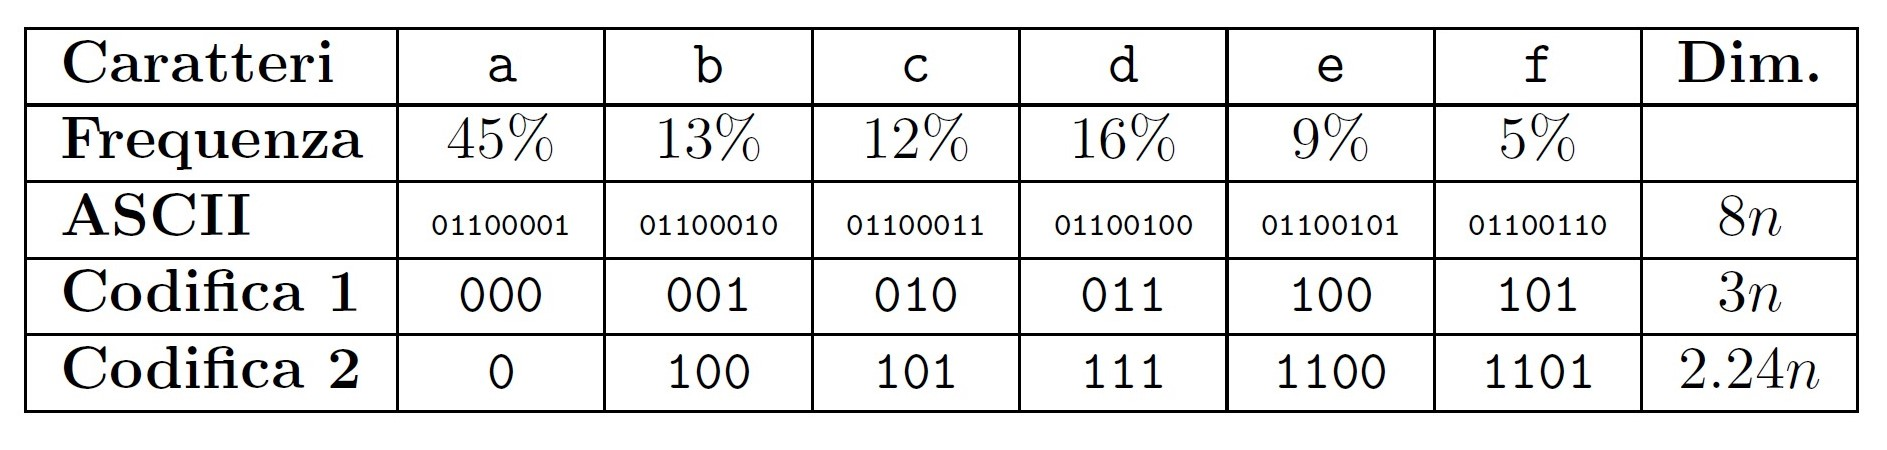
\includegraphics[width=0.8\textwidth]{../img/Greedy_1.jpg}
\caption{Possibili codifiche dei caratteri}
\end{figure} \\
Nella seguente immagine vengono mostrate codifiche differenti: la codifica ASCII estesa, una basata sui caratteri effettivamente presenti all'interno del testo mentre l'ultima basata sulla frequenza con cui compaiono i caratteri. L'ultimo caso è il più interessante poiché utilizza meno bit per memorizzare il carattere che compare più di frequente: questo viene definito \textcolor{red}{codice a prefissi}.\\
In un codice a prefisso, \textcolor{red}{nessun codice è un prefisso di un altro codice}. Ad esempio non è possibile mappare $a = 0$, $b = 1$, $c = 11$ poiché come interpreto poi 111111?
\newpage
\begin{flushleft}
\textbf{Rappresentazione ad albero per la decodifica}
\end{flushleft}
Un \textcolor{red}{albero binario di decodifica} viene così rappresentato
\begin{itemize}
	\item L'arco del figlio sinistro di ogni nodo è uno 0
	\item L'arco del figlio destro di ogni nodo è un 1
	\item Le sue foglie sono caratteri dell'alfabeto
\end{itemize}
\begin{figure}[h]
	\centering
	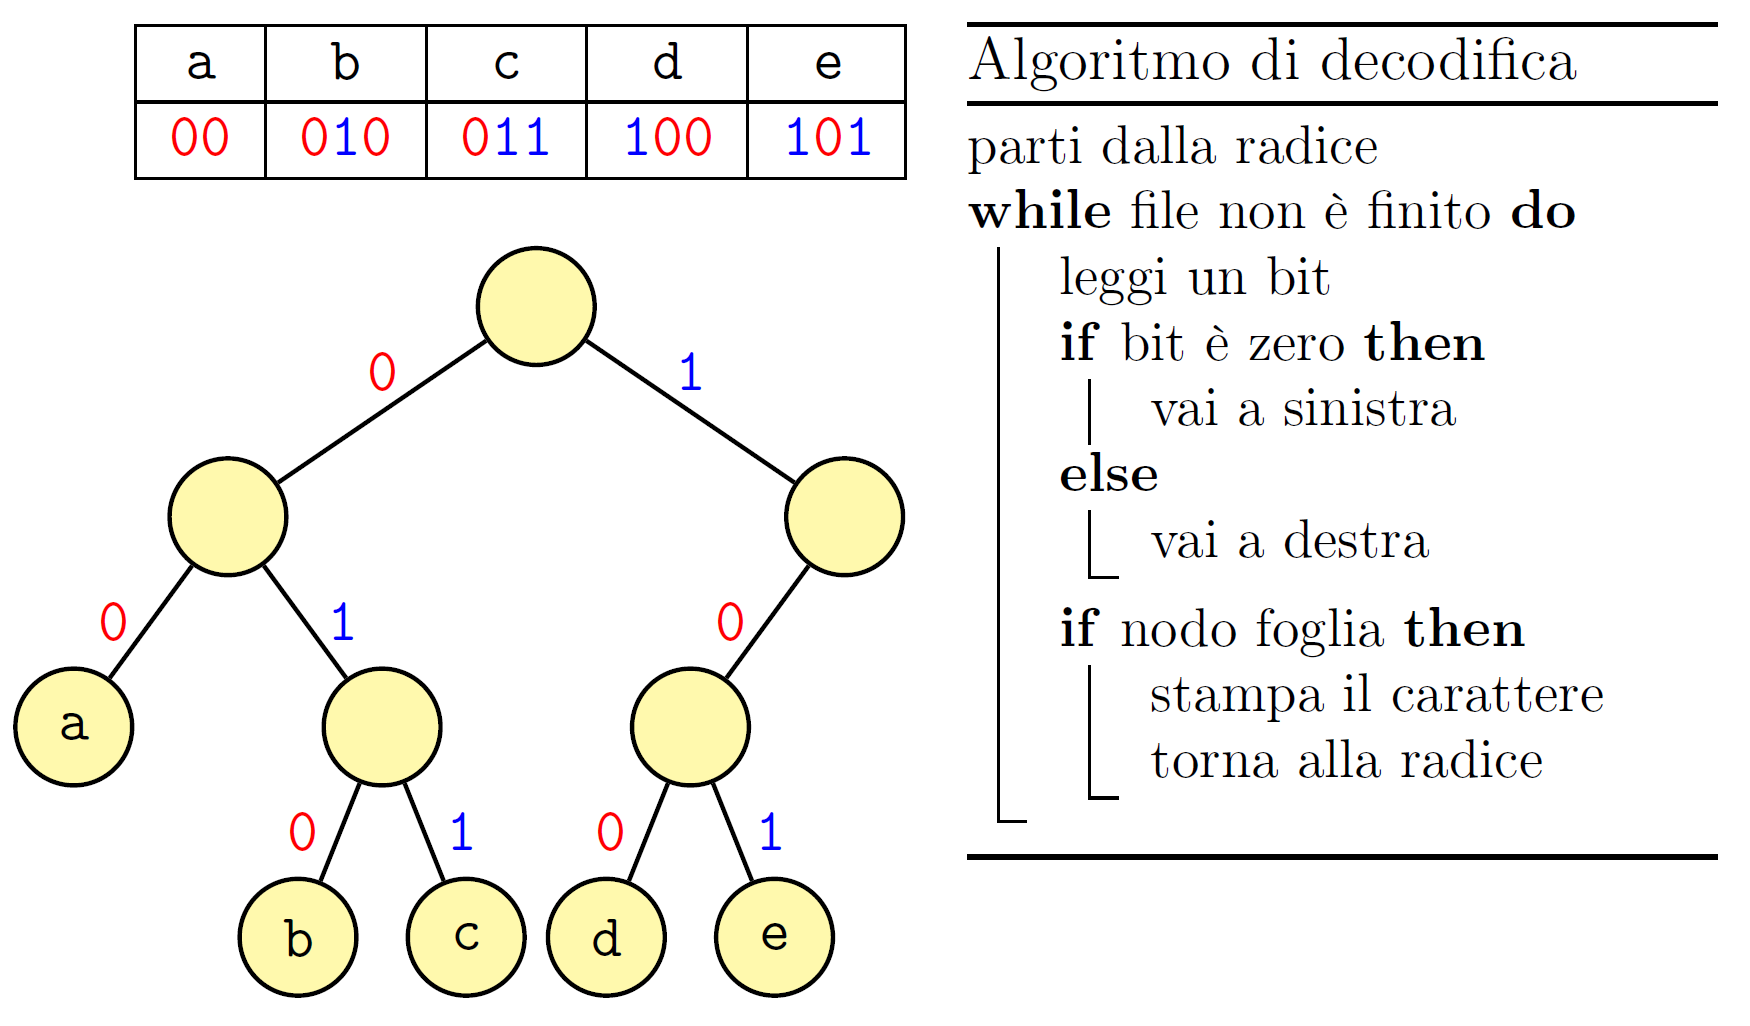
\includegraphics[width=0.7\textwidth]{../img/Greedy_2.png}
	\caption{Albero Binario di Decodifica - Rappresentazione}
\end{figure}
L'immagine precedente rappresenta un albero binario di decodifica che tuttavia ha un problema: il suo figlio destro infatti non serve a discriminare un carattere in particolare e quindi può essere tranquillamente tolto senza rendere la sequenza incomprensibile come nell'esempio precedente. Se quindi un nodo possiede un solo figlio all'interno di un albero binario di decodifica è possibile rimuovere il nodo e compattare l'albero.\\
\begin{figure}[h]
\centering
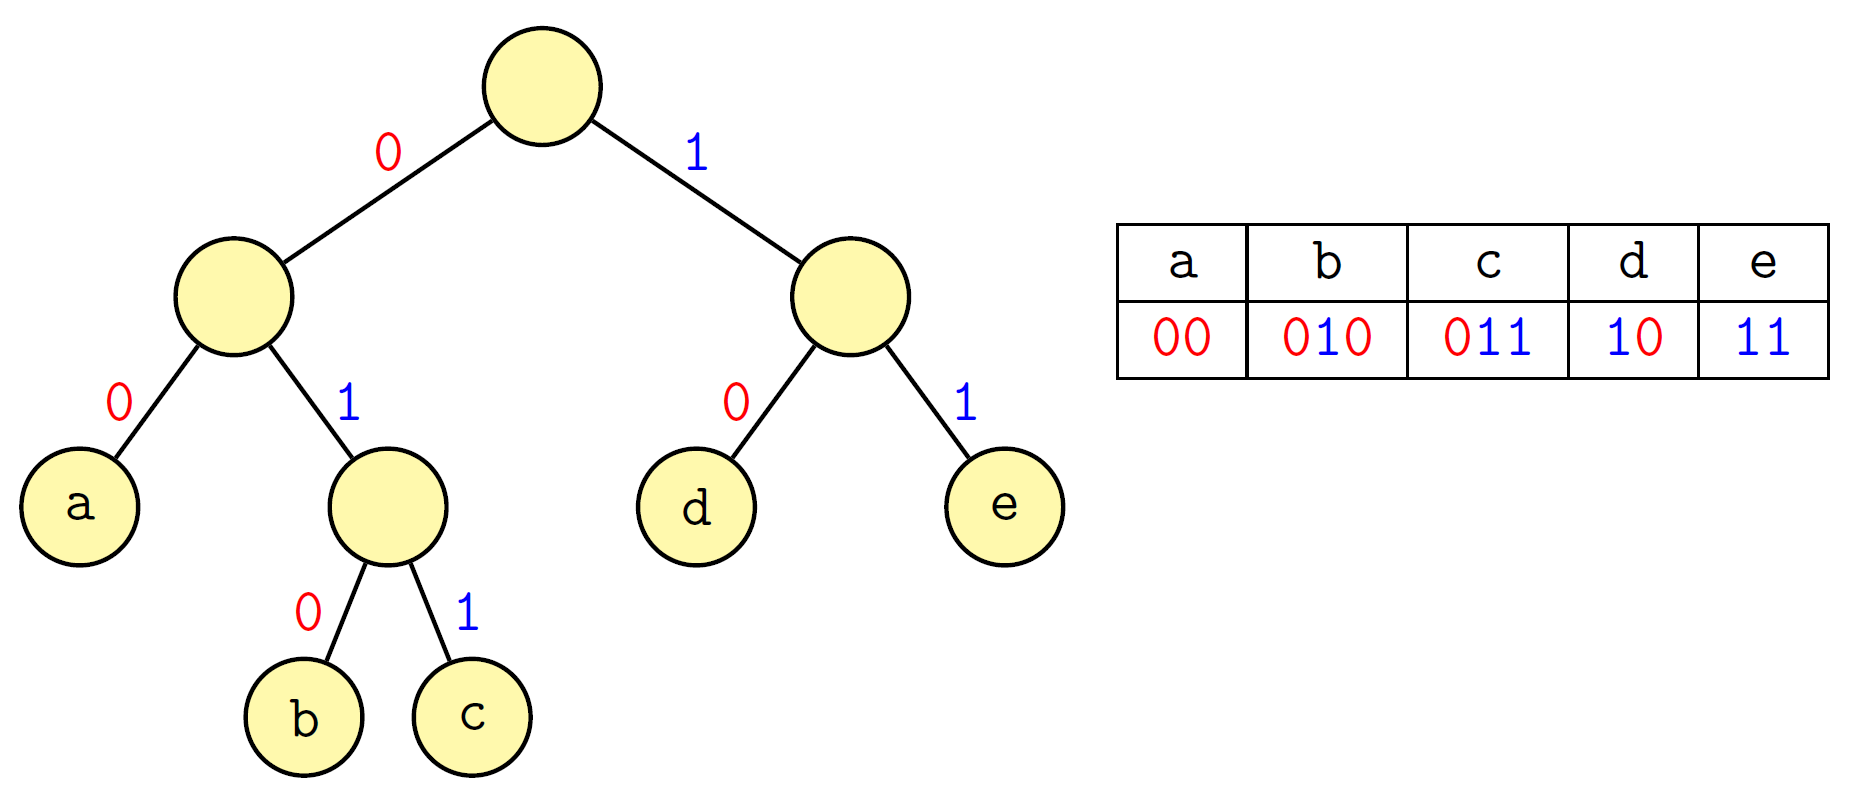
\includegraphics[width=0.7\textwidth]{../img/Greedy_3.png}
\caption{Albero Binario di Decodifica - Rimozione nodo}
\end{figure}
\newpage
\begin{flushleft}
\textbf{Definizione Formale del problema}
\end{flushleft}
Dato in input un file $F$ composto da caratteri nell'alfabeto $\mathcal{A}$, \textcolor{red}{quanti bit sono richiesti per codificare il file}?\\
Sia $T$ un albero che rappresenta la codifica e, per ogni $c \in \mathcal{A}$ (carattere dell'alfabeto), sia $d_{T}(c)$ la profondità della foglia che rappresenta $c$. Dagli schemi precedenti sappiamo che il codice per rappresentare $c$ richiederà allora $d_{T}(c)$ bit. Se $f[c]$ è il numero di occorrenze di $c$ in $F$, allora la dimensione della codifica è
\begin{center}
	$C[F, T] = \sum_{c \in \mathcal{A}} f[c] \cdot d_{T}(c)$
\end{center}
Il principio del \textbf{Codice di Huffman} è quello di minimizzare la lunghezza dei caratteri che compaiono più frequentemente assegnando di conseguenza ai caratteri con minore frequenza i percorsi più lunghi all'interno dell'albero. Ogni codice è progettato per un file specifico
\begin{itemize}
	\item Si ottiene la frequenza dei caratteri
	\item Si costruisce il codice
	\item Si rappresenta il file tramite il codice
	\item Si aggiunge al file una rappresentazione del codice, per la decodifica
\end{itemize}
\textbf{Funzionamento dell'algoritmo}
\begin{enumerate}
	\item Costruisci una lista ordinata di nodi foglia per ogni carattere in base alla loro frequenza
	\item Rimuovi i due nodi con frequenza minore $f_{x}$ e $f_{y}$
	\item Crea un nodo padre con etichetta - e frequenza $f_{x} + f_{y}$
	\item Collega i due nuovi rimossi con il nuovo nodo
	\item Aggiungi il nodo creato alla lista 
	\item Se la lista ha un solo elemento prosegui altrimenti ripeti da 2
	\item Etichetta gli archi dell'albero con bit 0, 1
\end{enumerate}
\begin{lstlisting}[caption=creazione albero binario di decodifica]
TREE huffman(int[] c, int f, int n)
	PRIORITYQUEUE Q = MinPriorityQueue()
	for i = 1 to n do
		% Creo i nodi dell'albero contenenti i caratteri
		Q.insert(f[i], Tree(f[i], c[i])
	% Fino a quando non ho un solo nodo
	for i = 1 to n - 1 do
		% Seleziono dalla lista i nodi con minore frequenza
		$z_{1}$ = Q.deleteMin()
		$z_{2}$ = Q.deleteMin()
		% Creo un nuovo nodo che ha come foglie i due nodi estratti
		$z$ = Tree($z_{1}$.f + $z_{2}$.f, nil)
		$z$.left = $z_{1}$
		$z$.right = $z_{2}$
		% Inserisco il nodo creato nella lista
		Q.insert($z$.f, $z$)
	return Q.deleteMin()
\end{lstlisting}
\subsection{Alberi di Copertura di peso minimo}
Dato un grafo pesato, determinare come interconnettere tutti i suoi nodi minimizzando il costo del peso associato ai suoi archi.
\begin{itemize}
	\item \textcolor{red}{Albero di copertura (di peso) minimo}
	\item \textcolor{red}{Albero di connessione (di peso) minimo}
	\item \textcolor{red}{Minimum spanning tree}
\end{itemize}
\textbf{Definizione del problema}\\
Viene dato in input un grafo \textcolor{red}{$G = (V, E)$} non orientato e connesso e  \textcolor{red}{$w: V \times V \rightarrow \mathbb{R}$} funzione di peso (costo di connessione) t.c. se $[u, v] \in E$, allora $w(u, v)$ è il peso dell'arco $[u, v]$, altrimenti $+\infty$. Poiché $G$ è \emph{non orientato}, $w(u, v) = w(v, u)$.\\\\
\textbf{Albero di Copertura (Spanning Tree)}\\
Dato un grafo $G = (V, E)$ non orientato e connesso, un \textcolor{red}{albero di copertura} di $G$ è un sottografo $T = (V, E_{T})$ tale che 
\begin{itemize}
	\item $T$ è un albero
	\item $E_{T} \subseteq E$
	\item $T$ contiene tutti i vertici di $G$
\end{itemize}
\textbf{Albero di copertura di peso minimo Vs Albero dei cammini minimi}
\begin{enumerate}
	\item Trovare l'albero di copertura il cui \textcolor{red}{peso totale} sia minimo rispetto a ogni altro albero di copertura, cioè per cui $w(T) = \sum_{[u, v] \in E_{T}}w(u, v)$ è minimo rispetto a tutti gli altri alberi di copertura
	\item Trovare l'albero di copertura con radice $v$ il cui \textcolor{red}{cammino da $v$ ad ogni altro vertice $u$} sia minimo
\end{enumerate}
In questa sezione ci occuperemo degli \textcolor{red}{Alberi di Copertura di Peso Minimo}, progettiamo dunque un algoritmo generico di tipo greedy per la risoluzione del problema e poi mostriamo le due istanze di tale algoritmo: \textcolor{red}{Kruskal} e \textcolor{red}{Prim}.\\
L'idea è quella di accrescere un sottoinsieme $A$ di archi in modo tale che venga sempre rispettata la seguente invariante:
\begin{itemize}
	\item $A$ è un sottoinsieme di qualche albero di connessione minimo
\end{itemize}
\textbf{Arco Sicuro}: Un arco $[u, v]$ è detto \textcolor{red}{sicuro per $A$} se $A \cup \{[u,v]\}$ è ancora un sottoinsieme di qualche albero di connessione minimo.
\begin{lstlisting}[caption=Algoritmo Generico MST]
SET mst-generico(GRAPH G, int[] w)
	SET A = $\emptyset$
	while A non forma un albero di copertura do
		trova un arco sicuro $[u, v]$
		A = A $\cup$ $\{[u, v]\}$
	return A
\end{lstlisting}
\newpage
\begin{flushleft}
\textbf{Definizioni}
\end{flushleft}
\begin{itemize}
	\item Un \textcolor{red}{taglio} $(S, V - S)$ di un grafo non orientato $G = (V, E)$ è una partizione di $V$ in due sottoinsiemi disgiunti
	\item Un arco $[u, v]$ \textcolor{red}{attraversa} il taglio se $u \in S$ e $v \in V - S$
	\item Un taglio \textcolor{red}{rispetta} un insieme di archi $A$ se nessun arco di $A$ attraversa il taglio
	\item Un arco che attraversa un taglio è \textcolor{red}{leggero} nel taglio se il suo peso è minimo fra i pesi degli archi che attraversano un taglio
\end{itemize}
\begin{figure}[h]
	\centering
	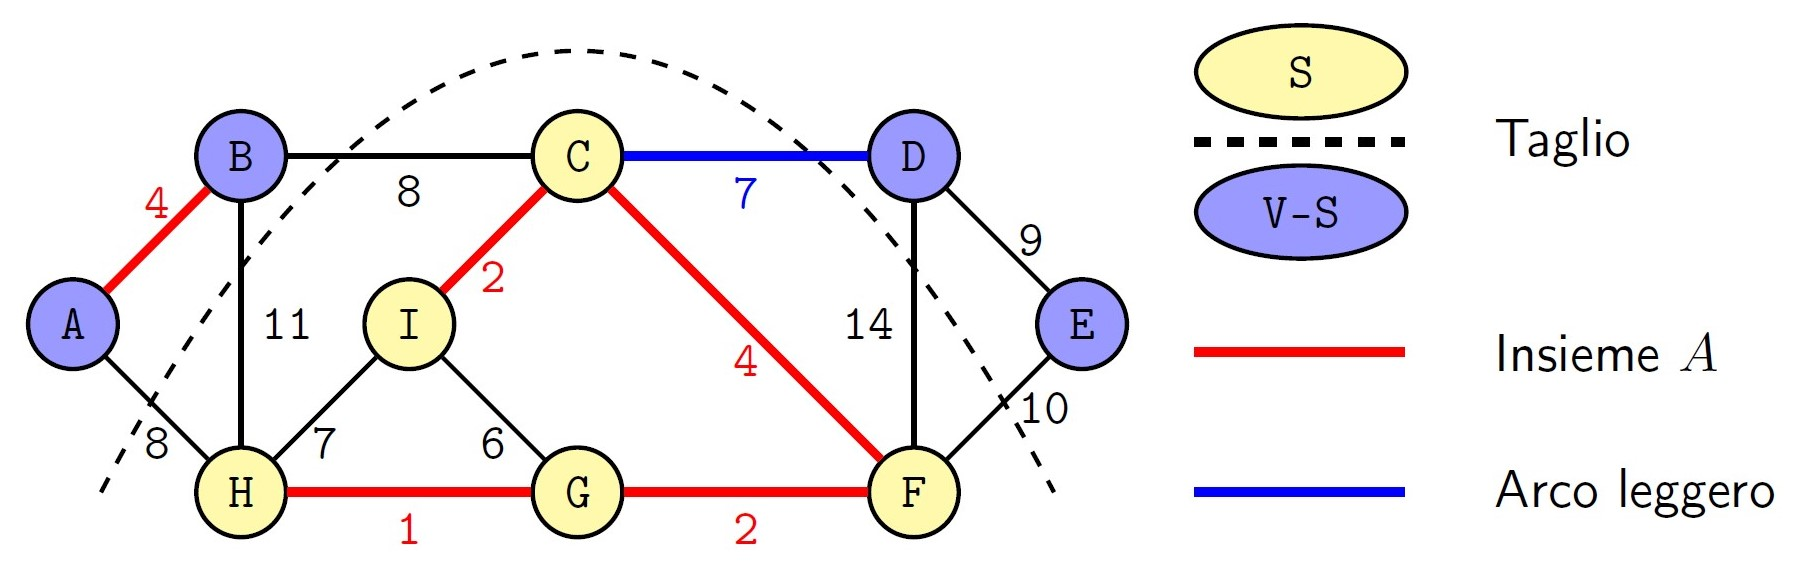
\includegraphics[width=0.7\textwidth]{../img/Greedy_4.jpg}
	\caption{Albero di copertura di peso minimo - Taglio}
\end{figure}
\textbf{Arco Sicuro: Teorema}
\begin{itemize}
	\item Sia $G = (V, E)$ un grafo \emph{non orientato} e $connesso$
	\item Sia $w$: $V \times V \rightarrow \mathbb{R}$
	\item Sia $A \subseteq E$ un sottoinsieme contenuto in qualche albero di copertura minimo per $G$
	\item Sia $(S, V - S)$ un qualunque taglio che rispetta $A$
	\item Sia $[u, v]$ un arco leggero che attraversa il taglio
\end{itemize}
Allora l'arco $[u, v]$ è \textcolor{red}{sicuro} per A\\\\
\textbf{Dimostrazione}\\
Sia $T$ un albero di copertura minimo che contiene $A$ e $(u, v)$ un arco leggero che attraversa il taglio (ha peso minimo tra tutti quelli che attraversano il taglio). Due casi:
\begin{itemize}
	\item $(u, v) \in T$: allora $(u, v)$ è sicuro per $A$
	\item $(u, v) \notin T$: trasformiamo $T$ in un albero $T'$ contenente $(u, v)$ e dimostriamo che $T'$ è un albero di copertura minimo
\end{itemize}
\newpage
\begin{flushleft}
\emph{Consideriamo la seguente situazione}:
\end{flushleft}
\noindent\begin{minipage}{0.3\textwidth}
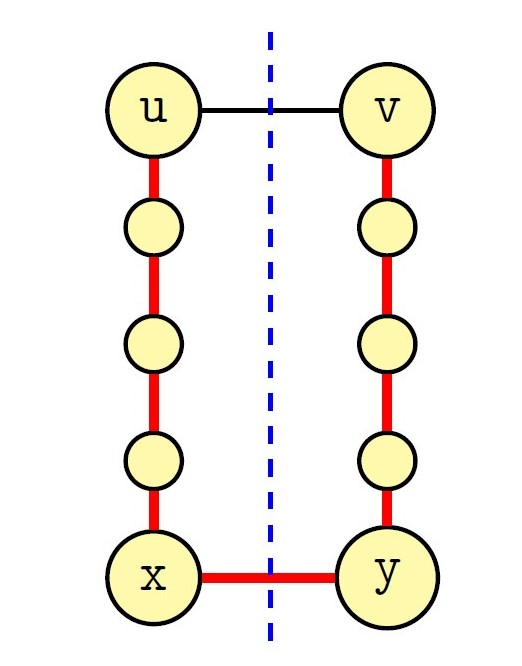
\includegraphics[width=\linewidth]{../img/Greedy_5.jpg}
\end{minipage}
\hfill
\begin{minipage}{0.6\textwidth}\raggedleft
\begin{itemize}
	\item $u, v$ sono connessi da un \textcolor{red}{cammino} $C \subseteq T$ (per definizione di albero)
	\item $u, v$ stanno in lati opposti del taglio (l'arco $(u, v)$ attraversa il taglio)
	\item $\exists (x, y) \in C$ che attraversa il taglio
\end{itemize}
\end{minipage}
\noindent\begin{minipage}{0.3\textwidth}
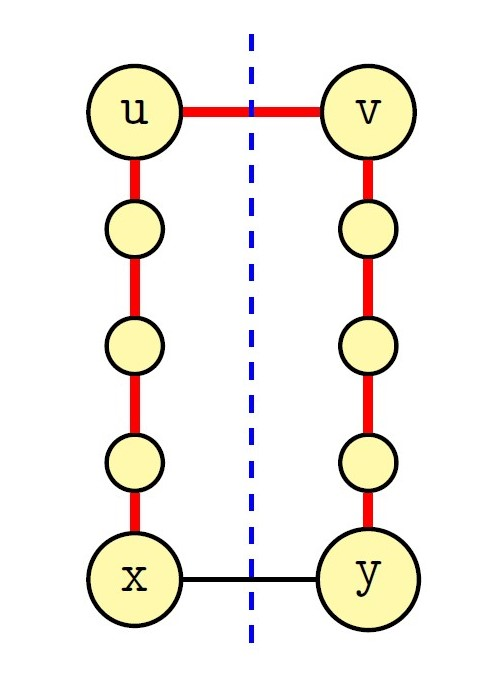
\includegraphics[width=\linewidth]{../img/Greedy_6.jpg}
\end{minipage}
\hfill
\begin{minipage}{0.6\textwidth}\raggedleft
\begin{itemize}
	\item $T' = T - \{(x, y)\} \cup \{(u, v)\}$
	\item $T'$ è un \emph{albero di copertura}
	\item $w(T') \leq w(T)$ (perché $w(u, v) \leq w(x, y)$)
	\item $w(T) \leq w(T')$ (perché $T$ minimo)
\end{itemize}
\end{minipage} \\\\
Dunque vale che $w(T') = w(T)$ e di conseguenza anche $T'$ è un albero di copertura di peso minimo.\\\\
\textbf{Corollario}
\begin{itemize}
	\item Sia $G = (V, E)$ un grafo \emph{non orientato} e $connesso$
	\item Sia $w$: $V \times V \rightarrow \mathbb{R}$
	\item Sia $A \subseteq E$ un sottoinsieme contenuto in qualche albero di copertura minimo per $G$
	\item Sia $C$ una componente connessa (un albero) nella foresta $G_{A} = (V, A)$
	\item Sia $[u, v]$ un arco leggero che connette $C$ a qualche altra componente in $G_{A}$
\end{itemize}
Allora l'arco $[u, v]$ è \textcolor{red}{sicuro} per A.\\\\
L'idea generale è di prendere una componente connessa $C$ nella foresta $G_{A}$ e un qualunque arco leggero $[u, v]$ che connette $C$ a qualche altra componente connessa di $G_{A}$ (di fatto anch'essa è un albero di peso minimo in quanto i suoi archi appartengono a un sottoinsieme contenuto in qualche albero di copertura di peso minimo). $[u, v]$ non può essere altro se un arco sicuro per $A$.
\newpage
\subsubsection{Algoritmo di Kruskal}
\textbf{Idea}
\begin{itemize}
	\item Ingrandire sottoinsiemi disgiunti di un albero di copertura minimo connettendoli fra di loro fino ad avere l’albero complessivo
	\item Si individua un arco sicuro scegliendo un arco $[u, v]$ di peso minimo tra tutti gli archi che connettono due alberi distinti (componenti connesse) della foresta
	\item L’algoritmo è greedy perché ad ogni passo si aggiunge alla foresta un arco con il peso minore
\end{itemize}
Per implementare l'algoritmo viene utilizzata la struttura dati \emph{Merge-Find Set} discussa nella sezione \emph{Strutture Dati Speciali} della dispensa
\begin{lstlisting}[caption=Albero di Copertura di Peso Minimo - Kruskal]
SET kruskal(EDGE[] A, int n, int m)
	SET T = Set()
	MFSET M = Mfset(n)
	$\{$ordina $A[1...m]$ in modo che $A[1].weight \leq ... \leq A[m].weight\}$
	% Archi totali
	int count = 0
	% Arco che sto considerando
	int i = 1
	% Temina qunado l'albero ha n - 1 archi o non ci sono altri archi
	while count < n-1 and i $\leq$ m do
		% Controllo se i nodi dell'arco non appartengono allo stesso insieme
		if M.find(A[i].u) $\neq$  M.find(A[i].v) then
			% in quel caso li metto nello stesso insieme
			M.merge(A[i].u, A[i].v)
			% e aggiungo l'arco all'insieme degli archi del mst
			T.insert(A[i])
			count = count + 1
		i = i + 1
	return T
\end{lstlisting}
\textbf{Analisi della complessità algoritmo di Kruskal}\\
Il tempo di esecuzione per l'algoritmo di Kruskal dipende dalla realizzazione della struttura dati per Merge-Find Set: se utilizziamo la versione con \textcolor{red}{euristica sul rango + compressione}, (*) le cui operazioni hanno costo ammortizzato costante otteniamo
\begin{center}
	\renewcommand{\arraystretch}{1.2}
	\begin{tabular}{ |c|c|c| } 
		\hline
			\textbf{Fase} & \textbf{Volte} & \textbf{Costo}\\ 
		\hline
			Inizializzazione & 1 &  $\mathcal{O}(n)$\\ 
		\hline
			Ordinamento & 1 &  $\mathcal{O}(m \log m)$ \\
		\hline
			Operazioni \textbf{find}(), \textbf{merge}() & $\mathcal{O}(m)$ & $\mathcal{O}(1)^{(*)}$\\
		\hline
	\end{tabular}
\end{center}
Complessivamente dunque il costo dell'algoritmo sarà dato da $\mathcal{O}(n + m \log m + m) = \mathcal{O}(m \log m)$\\
Sappiamo però che $m$, il numero totale degli archi che compongono il nostro grafo, può essere al massimo pari a $n-1$ per ogni nodo nel caso di un grafo completo: questo significa un totale di $n^{2}$ archi. La complessità può essere sostanzialmente riscritta come $\mathcal{O}(m \log n^{2})$.\\
Per le proprietà degli logaritmi possiamo però a questo punto portare all'esterno il 2 all'esponente che, diventando una costante, può essere tranquillamente ignorato e la complessità finale risulta dunque essere \textcolor{red}{$\mathcal{O}(m \log n)$}.
\newpage
\begin{flushleft}
\textbf{Evoluzione algoritmo di Kruskal - Esempio}
\end{flushleft}
\begin{figure}[h]
	\centering
	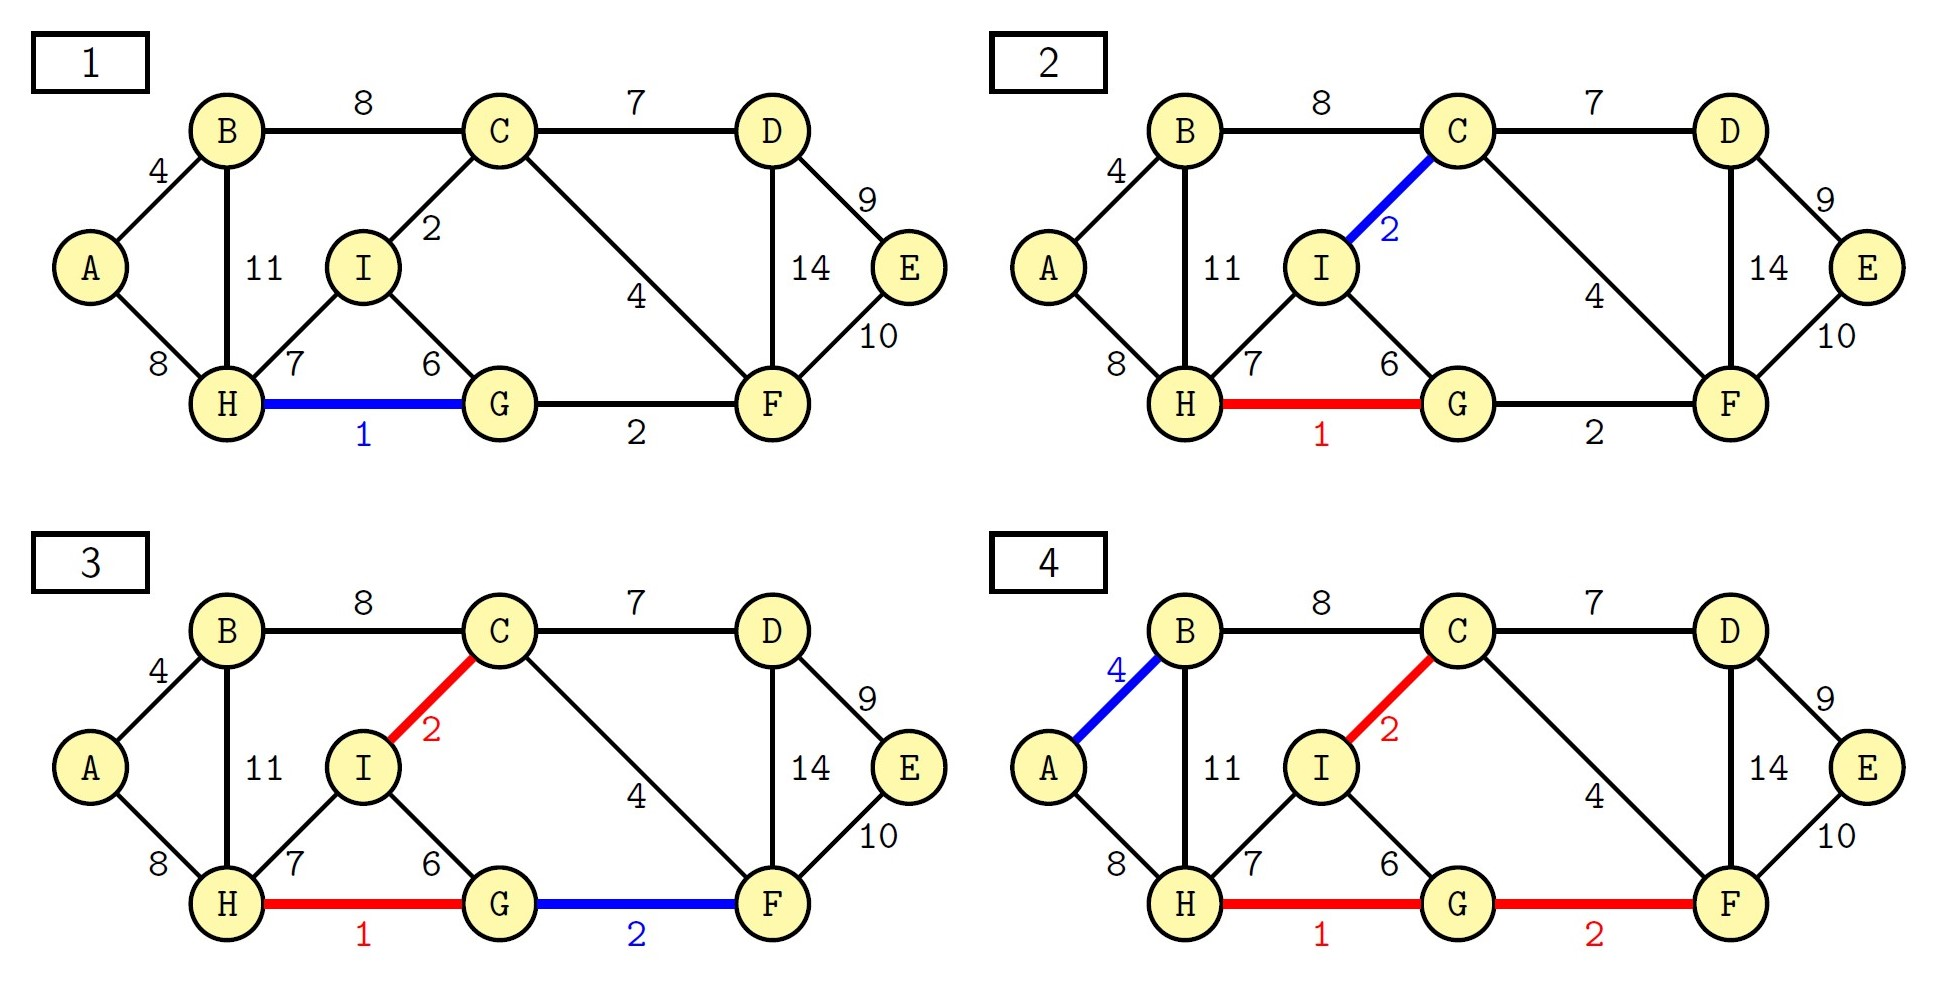
\includegraphics[width=0.7\textwidth]{../img/Greedy_7.jpg}
	\caption{Evoluzione algoritmo di Kruskal - 1..4}
\end{figure}
\begin{figure}[h]
	\centering
	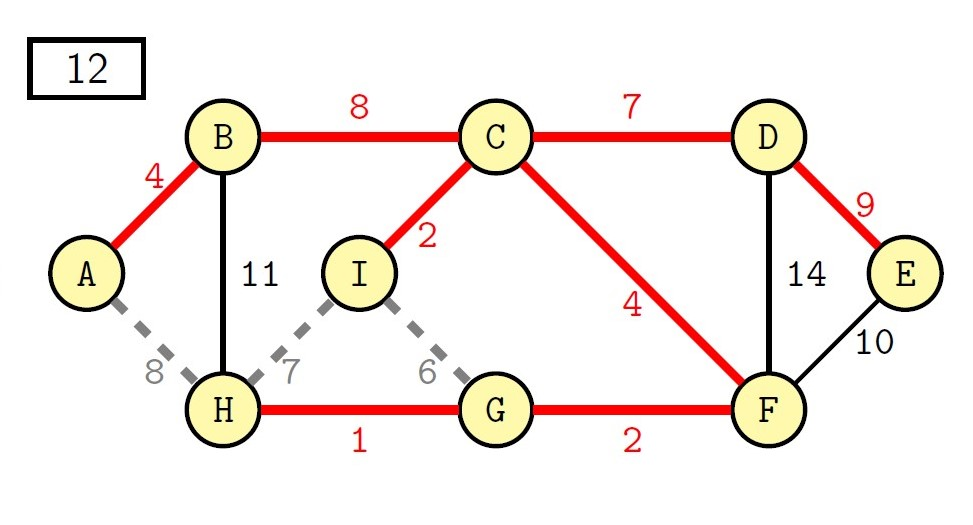
\includegraphics[width=0.5\textwidth]{../img/Greedy_8.jpg}
	\caption{Evoluzione algoritmo di Kruskal - Completo}
\end{figure}
Come si può osservare alcuni gli archi 6, 7 e 8 archi nell'immagine completa sono colorati in grigio in quanto sono stati estratti prima dell'arco 9 poiché di peso minore, tuttavia sono stati scartati in quanto l'operazione di find del Merge-Find Set ha restituito il medesimo rappresentante in quanto i due nodi facevano già parte dell'albero di copertura di peso minimo creato nel corso dell'algoritmo. Gli archi 10, 11 e 14 non sono stati analizzati invece poichè sono stati raggiunti gli $n-1$ archi che costruiscono l'albero.
\newpage
\subsubsection{Algoritmo di Prim}
\textbf{Idea}
\begin{itemize}
	\item L'algoritmo di Prim procede mantenendo in $A$ un singolo albero
	\item L'albero parte da un vertice arbitrario $r$ (la radice) e cresce fino a quando non ricopre tutti i vertici
	\item Ad ogni passo viene aggiunto un \emph{arco leggero} che collega un vertice in $V_{A}$ con un vertice in $V - V_{A}$, dove $V_{A}$ è l'insieme di nodi raggiunti da archi in $A$
\end{itemize}
Per definizione $(V_{A}, V - V_{A})$ è un taglio che rispetta $A$ (infatti $V_{A}$ contiene i nodi connessi da archi appartenenti ad $A$ mentre $V-V_{A}$ quelli che ancora devono essere raggiunti dunque nessun arco di $A$ può attraversare il taglio) e per il corollario esposto precedentemente gli archi leggeri che attraversano il taglio sono sicuri.\\\\
\textbf{Implementazione}\\
La struttura dati che si utilizza in questo caso è una \emph{Min Priority Queue} la cui descrizione e implementazione si può trovare nella sezione \emph{Strutture Dati Speciali} della dispensa. Durante l'esecuzione, i vertici non ancora nell'albero si trovano in una coda con min-priorità $Q$ ordinata in base alla seguente definizione di priorità: la priorità del nodo $v$ è il peso minimo di un arco che collega $v$ ad un vertice nell'albero, o +$\infty$ se tale arco non esiste.\\
L'implementazione dell'albero avviene invece tramite \emph{vettore dei padri} di conseguenza
\begin{itemize}
	\item Ogni nodo $v$ mantiene un puntatore al padre $p[v]$
	\item $A$ è mantenuto implicitamente: $A = \{[v, p[v]] \mid v \in V - Q - \{r\}\}$ ($r$ non può essere selezionato come nodo in quanto è il nodo radice dell'albero e non può avere un padre)
\end{itemize}
\begin{lstlisting}[caption=Albero di Copertura di Peso Minimo - Prim]
prim(GRAPH G, NODE r, int[] p)
	PRIORITYQUEUE Q = MinPriorityQueue()
	% Creiamo i Priority Item per accedere ad un elemento piu' in fretta
	PRIORITYITEM[] pos = new PRIORITYITEM[1...G.n]
	% Inserisco tutti gli archi con priorita' +infinito tranne r
	foreach u $\in$ G.V() - $\{$r$\}$ do
		pos[u] = Q.insert(u, +$\infty$)
	% Inseriamo la radice con priorita' 0
	pos[r] = Q.insert(r, 0)
	% Impostiamo il suo padre a 0
	p[r] = 0
	while not Q.isEmpty() do
		% preleviamo il nodo con minore priorita' (caso base = r)
		NODE u = Q.deleteMin()
		% impostiamo l'elemento a nil nei priority item
		pos[u] = nil
		% controlliamo gli archi v adiacenti a u
		foreach v $\in$ G.adj(u) do
			% se non ho gia' estratto il nodo e se un arco ha peso minore della priorita' 
			if pos[v] $\neq$ nil and w(u, v) $<$ pos[v].priority then
				% la sua priorita' diventa il peso dell'arco
				Q.decrease(pos[v], w(u, v))
				% imposto suo padre ad u
				p[v] = u
\end{lstlisting}
\textbf{Analisi della complessità algoritmo di Prim}\\
L'efficienza dell'algoritmo di Prim dipende dall'implementazione della coda con priorità, se si utilizza un \emph{Heap Binario}
\begin{center}
	\renewcommand{\arraystretch}{1.2}
	\begin{tabular}{ |c|c|c| } 
		\hline
			\textbf{Fase} & \textbf{Volte} & \textbf{Costo}\\ 
		\hline
			Inizializzazione & 1 &  $\mathcal{O}(n \log n)$\\ 
		\hline
			\textbf{deleteMin}() & $\mathcal{O}(n)$ &  $\mathcal{O}(\log n)$ \\
		\hline
			\textbf{decreasePriority}() & $\mathcal{O}(m)$ & $\mathcal{O}(\log n)$\\
		\hline
	\end{tabular}
\end{center}
Il tempo totale è dunque $\mathcal{O}(n + n \log n + m \log n) = \textcolor{red}{\mathcal{O}(m \log n)}$ e quindi è asintoticamente uguale a quello di Kruskal.\\
Se la coda con priorità fosse invece implementata tramite \emph{vettore non ordinato} il costo diventerebbe $\mathcal{O}(n^{2})$.\\
La scelta del tipo di struttura da utilizzare dipende dal tipo di grafo in questione se \emph{sparso} oppure \emph{fortemente connesso}.\\\\
\textbf{Evoluzione algoritmo di Prim - Esempio}
\begin{figure}[h]
	\centering
	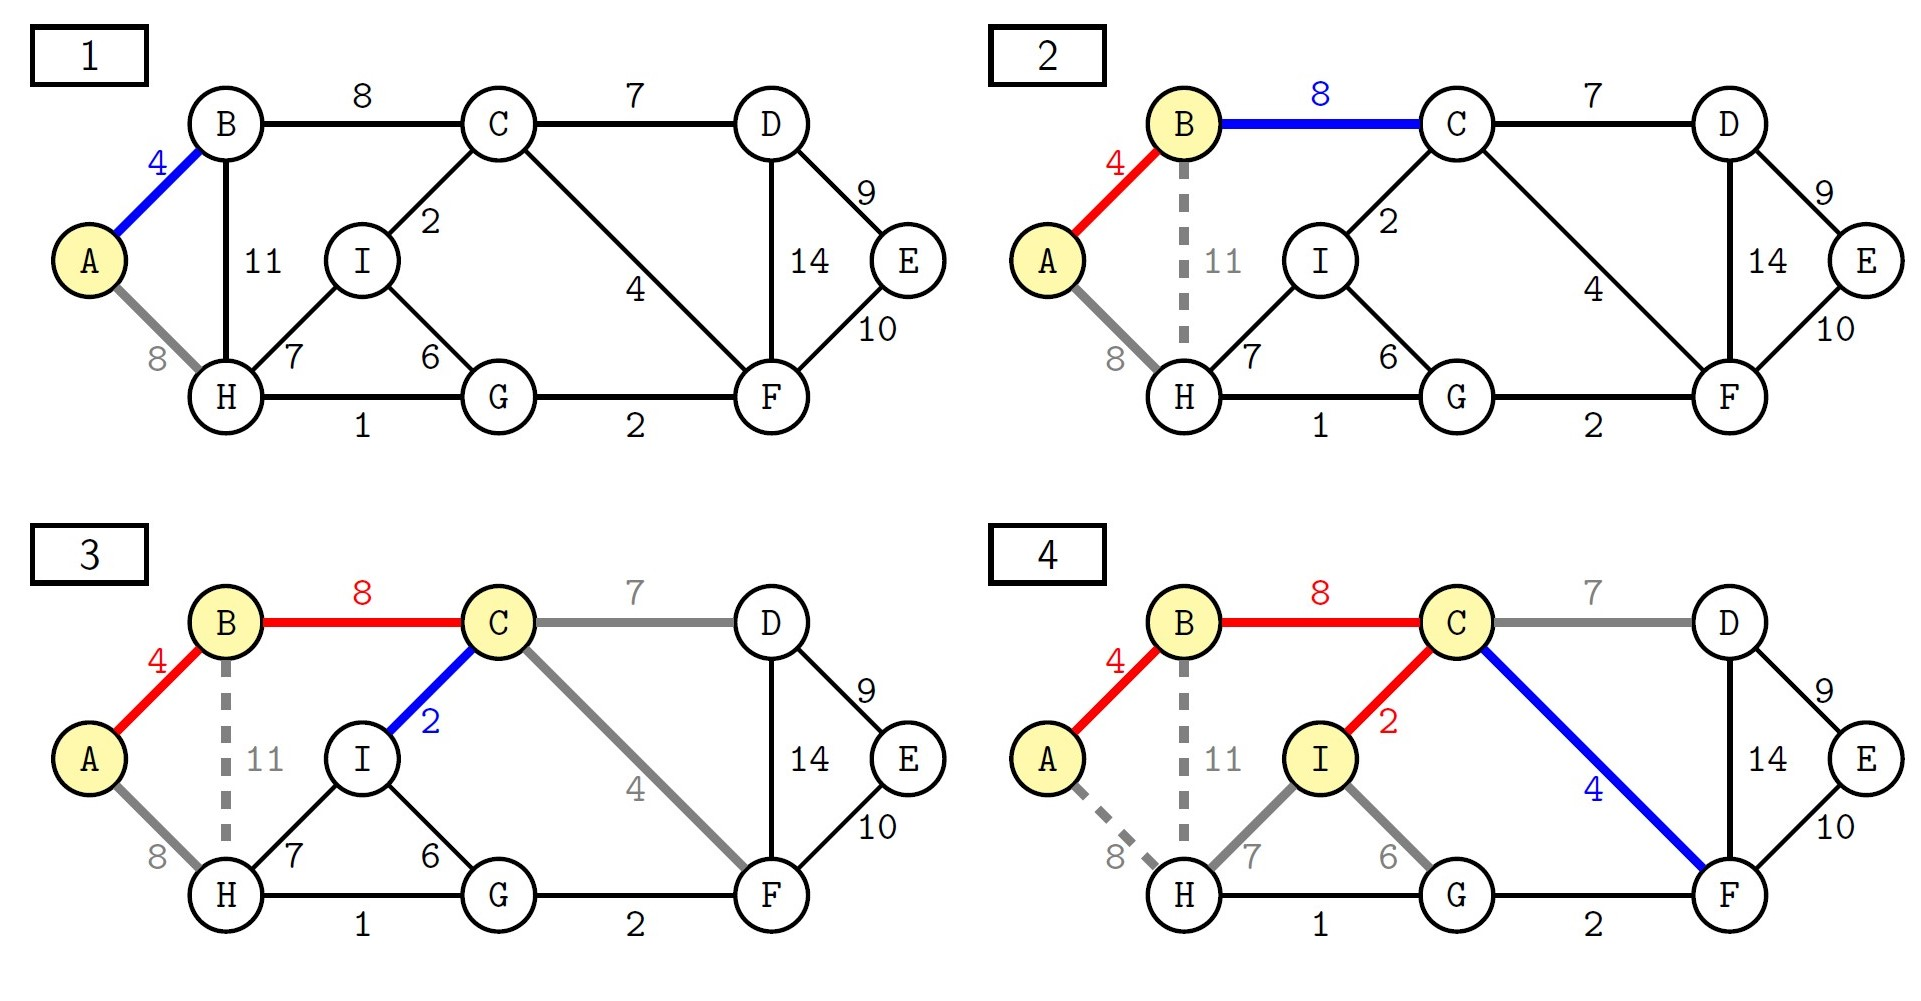
\includegraphics[width=0.7\textwidth]{../img/Greedy_9.jpg}
	\caption{Evoluzione algoritmo di Prim - 1..4}
\end{figure}
\begin{figure}[h]
	\centering
	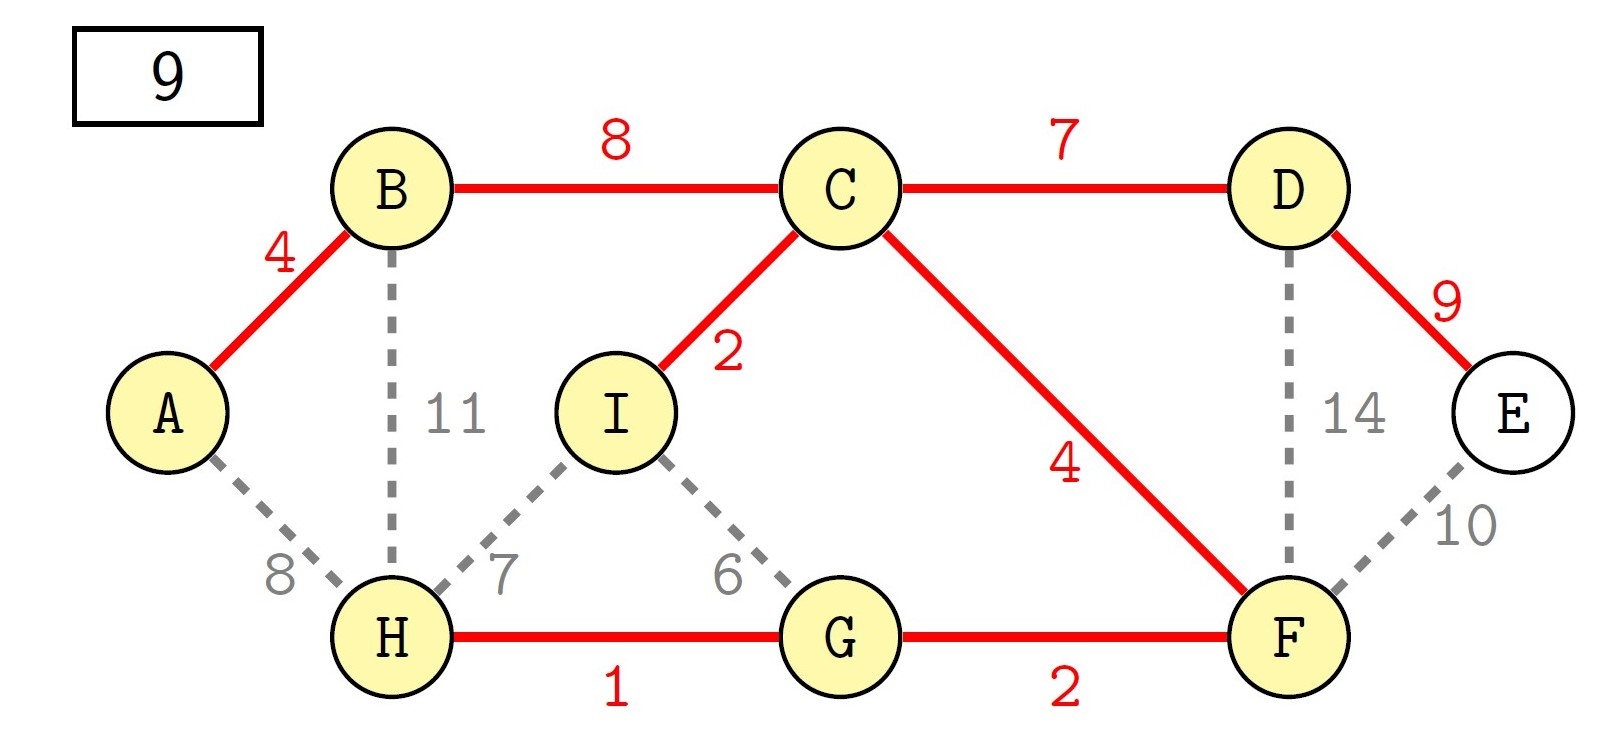
\includegraphics[width=0.5\textwidth]{../img/Greedy_10.jpg}
	\caption{Evoluzione algoritmo di Prim - Completo}
\end{figure} \\
Nel caso dell'algoritmo di Prim gli archi che si vanno a considerare seguono come logica quello dell'ultimo arco aggiunto. Gli archi colorati di grigio (non tratteggiati) indicano quelli che sono stati analizzati dall'algoritmo e la cui priorità è stata modificata ma non è detto che saranno quelli che verranno usati per formare l'albero di copertura di peso minimo.
\newpage
\end{document}
